
\section{Анализ задач разгона и торможения в контексте системы управления}\label{sec:ch1/sec5}
В настоящее время, благодаря стремительному развитию микроэлектроники и её применению в различных
областях, стало возможным использование сложных алгоритмов управления. Эти достижения позволяют решать
вопросы, которые были исследованы ранее, при помощи разнообразных алгоритмов управления.

Однако применение алгоритмов управления, предназначенных для непрерывных систем, к системам с
дискретными элементами может быть затруднительным или даже невозможным. Для использования
ПИД-регулятора исследователи применяют различные преобразователи и модуляции сигнала. Например,
широко распространено использование широтно-импульсной модуляции (ШИМ) в сочетании с ПИД.

Аналогично, инженеры используют разнообразные интеллектуальные алгоритмы управления на основе
нейросетей или нечёткой логики. Также особую популярность получило управление в скользящих режимах,
которое зарекомендовало себя в управлении электроприводом. Это связано с тем, что модель представляет
собой дискретную систему.

\subsection{Исследование управления с использованием ШИМ}\label{subsec:ch1/sec5/subsec1}

В работе \cite*{pwm:Varseveld} подробно рассмотрена разработка системы позиционного ПП, схема которого представлена на
рисунке \ref*{fig:позиционный_пп_pwm}, с использованием недорогих
дискретных распределителей с электромагнитным управлением, вместо дорогостоящих пропорциональных. Особое внимание уделено
проектированию системы управления, обеспечивающей высокое быстродействие и точность позиционирования.

\begin{figure}[htpb]
    \centerfloat
    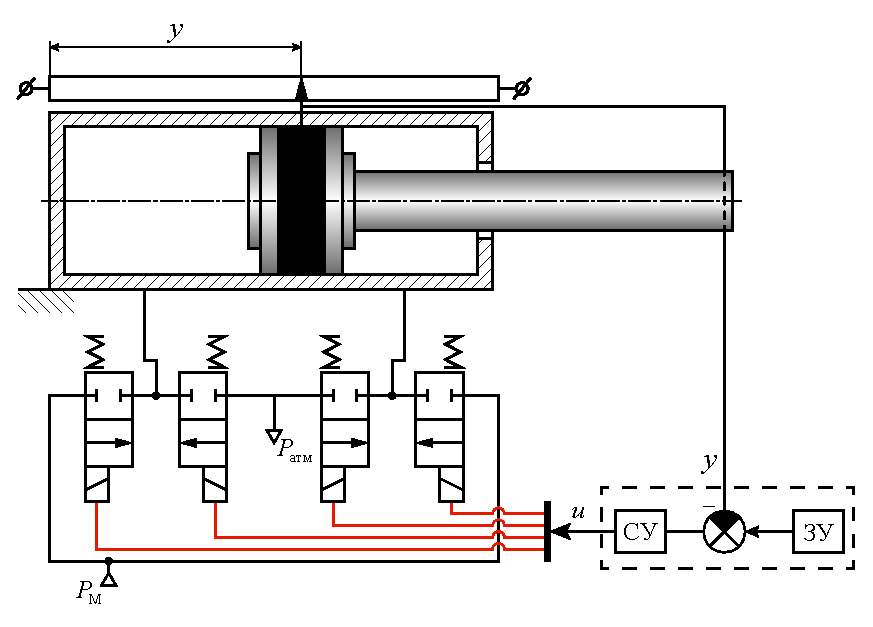
\includegraphics{positioning_actuator_pwm_ov.eps}
    \caption{Схема позиционного ПП с дискретными распределителями}\label{fig:позиционный_пп_pwm}
\end{figure}

Авторами предложен новый алгоритм с использованием широтно-импульсной модуляции (ШИМ) для управления распределителями, позволяющий
получить практически симметричную и линейную характеристику скорости РО ПП в зависимости от управляющего сигнала.
Это достигается за счет согласованного управления магистральными и выхлопными распределителями, что компенсирует асимметрию,
вызванную разницей активных площадей поршня в поршневой и штоковой полостях. Экспериментальные исследования подтвердили высокую линейность и
симметрию полученной характеристики.

На основе экспериментальных данных авторами синтезирована линейная авторегрессионная модель ПП.
Анализ модели показал, что демпфирование системы существенно зависит от положения поршня, достигая минимума в
центральной части хода. Это объясняется наличием сухого кулоновского трения.

Для компенсации влияния трения в систему управления введен ПИД-регулятор с дополнительной компенсацией
трения и интегральной составляющей ограниченной с двух сторон. Применение этих мер позволило существенно уменьшить статическую
ошибку позиционирования.

В ходе экспериментальных исследований авторам удалось достичь высокого быстродействия системы управления --
время нарастания составило всего 180~\si{\milli\second}. При этом статическая ошибка позиционирования не превышала 0,21~
\si{\milli\metre},
что сопоставимо с результатами, полученными другими исследователями
\cite*{Varseveld:article1,Varseveld:article2,Varseveld:article3,Surgenor1997ContinuousSM},
использовавшими более дорогостоящие
пропорциональные распределители. Кроме того, система продемонстрировала инвариантность к шестикратному изменению
инерционной нагрузки. Авторы также показали возможность точного отслеживания $S$-образных траекторий с ошибкой не
более 2~\si{\milli\metre}.

Статья \cite*{Shiee} посвящена сравнительному анализу различных схем ШИМ для улучшения позиционирования ПП. Авторы рассматривают пять
основных ШИМ-схем представленных на рисунке \ref*{fig:схемы_шим}.

\begin{figure}[ht]
    \centerfloat{
        \subcaptionbox[List-of-Figures entry]{\label{fig:схемы_шим-1}}{
            \begin{tikzpicture}
                \begin{axis}[
                        width = 8cm,
                        height = 5cm,
                        xmin=-100, xmax=100,
                        ymin=0, ymax=100,
                        xlabel={Сигнал, \%},
                        ylabel={Ширина ШИМ, \%},
                        grid=major,
                        extra tick style={grid=none, draw opacity=0},
                        tick style={line width=0.75pt},
                        axis line style={line width=1pt},
                    ]
                    \addplot[black, mark=none, line width=0.75pt] coordinates {
                            (-100, 0)
                            (100, 100)
                        };
                    \addplot[black, mark=none, line width=0.75pt, dashed] coordinates {
                            (-100, 100)
                            (100, 0)
                        };
                    %add legend
                    \addlegendentry{Расп. 1}
                    \addlegendentry{Расп. 2}


                \end{axis}
            \end{tikzpicture}
        }
        \hfil
        \subcaptionbox[]{\label{fig:схемы_шим-2}}{
            \begin{tikzpicture}
                \begin{axis}[
                        width = 8cm,
                        height = 5cm,
                        xmin=-100, xmax=100,
                        ymin=0, ymax=100,
                        xlabel={Сигнал, \%},
                        ylabel={Ширина ШИМ, \%},
                        grid=major,
                        extra tick style={grid=none, draw opacity=0},
                        tick style={line width=0.75pt},
                        axis line style={line width=1pt},
                    ]
                    \addplot[black, mark=none, line width=0.75pt] coordinates {
                            (-100, 10)
                            (-80, 10)
                            (80, 80)
                            (100, 100)
                        };
                    \addplot[black, mark=none, line width=0.75pt, dashed] coordinates {
                            (-100, 100)
                            (-80, 80)
                            (80, 10)
                            (100, 10)
                        };
                    %add legend
                    \addlegendentry{Расп. 1}
                    \addlegendentry{Расп. 2}


                \end{axis}
            \end{tikzpicture}
        }
        \vfil
        \subcaptionbox[]{\label{fig:схемы_шим-3}}{
            \begin{tikzpicture}
                \begin{axis}[
                        width = 8cm,
                        height = 5cm,
                        xmin=-100, xmax=100,
                        ymin=0, ymax=100,
                        xlabel={Сигнал, \%},
                        ylabel={Ширина ШИМ, \%},
                        grid=major,
                        extra tick style={grid=none, draw opacity=0},
                        tick style={line width=0.75pt},
                        axis line style={line width=1pt},
                    ]
                    \addplot[black, mark=none, line width=0.75pt] coordinates {
                            (-100, 20)
                            (-70, 20)
                            (70, 80)
                            (100, 80)
                        };
                    \addplot[black, mark=none, line width=0.75pt,dashed] coordinates {
                            (-100, 80)
                            (-70, 80)
                            (70, 20)
                            (100, 20)
                        };
                    %add legend
                    \addlegendentry{Расп. 1}
                    \addlegendentry{Расп. 2}
                \end{axis}
            \end{tikzpicture}
        }
        \hfil
        \subcaptionbox[]{\label{fig:схемы_шим-4}}{
            \begin{tikzpicture}
                \begin{axis}[
                        width = 8cm,
                        height = 5cm,
                        xmin=-100, xmax=100,
                        ymin=0, ymax=100,
                        xlabel={Сигнал, \%},
                        ylabel={Ширина ШИМ, \%},
                        grid=major,
                        extra tick style={grid=none, draw opacity=0},
                        tick style={line width=0.75pt},
                        axis line style={line width=1pt},
                    ]
                    \addplot[black, mark=none, line width=0.75pt, ] coordinates {
                            (-100, 20)
                            (0, 20)
                            (100, 80)
                        };
                    \addplot[black, mark=none, line width=0.75pt, dashed] coordinates {
                            (-100, 80)
                            (0, 20)
                            (100, 20)
                        };
                    %add legend
                    \addlegendentry{Расп. 1}
                    \addlegendentry{Расп. 2}
                \end{axis}
            \end{tikzpicture}
        }
        \vfil    \subcaptionbox[]{\label{fig:схемы_шим-5}}{
            \begin{tikzpicture}
                \begin{axis}[
                        width = 8cm,
                        height = 5cm,
                        xmin=-100, xmax=100,
                        ymin=0, ymax=100,
                        xlabel={Сигнал, \%},
                        ylabel={Ширина ШИМ, \%},
                        grid=major,
                        extra tick style={grid=none, draw opacity=0},
                        tick style={line width=0.75pt},
                        axis line style={line width=1pt},
                    ]
                    \addplot[black, mark=none, line width=0.75pt, ] coordinates {
                            (-100, 20)
                            (0, 80)
                            (100, 80)
                        };
                    \addplot[black, mark=none, line width=0.75pt, dashed] coordinates {
                            (-100, 80)
                            (0, 80)
                            (100, 20)
                        };
                    %add legend
                    \addlegendentry{Расп. 1}
                    \addlegendentry{Расп. 2}
                \end{axis}
            \end{tikzpicture}
        }
    }
    \caption{Схемы ШИМ}\label{fig:схемы_шим}
\end{figure}

Схема \cref*{fig:схемы_шим-1} не учитывает динамику включения/выключения распределителей, что приводит к нелинейностям при
крайних значениях входного сигнала. Схема \cref*{fig:схемы_шим-2} учитывает только динамику включения распределителей и добавляет точку перегиба,
чтобы минимизировать ширину импульса ниже определенного значения. Схема \cref*{fig:схемы_шим-3} учитывает как задержку включения, так и
задержку выключения распределителей, вводя два пограничных значения для ширины импульса. Схема \cref*{fig:схемы_шим-4} является модифицированным
вариантом схемы \cref*{fig:схемы_шим-1}, учитывающим задержки клапанов, и обеспечивает меньшую сумму коэффициентов заполнения сигнала поступающего на распределитель,
особенно вблизи нулевого входного сигнала. Схема \cref*{fig:схемы_шим-5} представляет собой модификацию схемы \cref*{fig:схемы_шим-3} с
учетом задержек включения
и выключения клапанов, давая большую суммарную ширину импульса вблизи нулевого входа.

Авторы провели ряд экспериментов со ступенчатыми и гармоническими входными воздействиями, чтобы изучить характеристики
различных ШИМ-схем. По характеристикам позиционирования при ступенчатом входе, схема \cref*{fig:схемы_шим-1} показала наименьшее время
нарастания, но большую статическую ошибку позиционирования, схема \cref*{fig:схемы_шим-4} продемонстрировала наименьшее перерегулирование,
но худшую ошибку, а схема \cref*{fig:схемы_шим-5} имела самое большое время нарастания и ошибку.
При отслеживании гармонического сигнала, первые три схемы показали близкие результаты по среднеквадратичной
ошибке, в то время как схемы \cref*{fig:схемы_шим-4} и \cref*{fig:схемы_шим-5} имели большую ошибку слежения. Эксперименты с увеличением нагрузки показали,
что схема \cref*{fig:схемы_шим-4}
оказалась наименее устойчивой к увеличению инерционной нагрузки, а схема \cref*{fig:схемы_шим-5}, имеющая высокое рабочее давление,
продемонстрировала наибольшую
устойчивость.

Чтобы компенсировать влияние различий в эффективных площадях, авторы предложили модифицированные версии каждой ШИМ-схемы.
Модификация заключается в сдвиге диаграмм ШИМ-схем с целью достижения нулевой выходной силы при нулевом входном сигнале.

Экспериментальные результаты при ступенчатом входном воздействии продемонстрировали, что модифицированные ШИМ-схемы, особенно для схем \cref*{fig:схемы_шим-1},
\cref*{fig:схемы_шим-2}, \cref*{fig:схемы_шим-3} и \cref*{fig:схемы_шим-5}, обеспечивают значительное улучшение характеристик позиционирования,
в частности, снижение статической ошибки позиционирования. Это связано с тем, что при высоких рабочих давлениях различия в эффективных площадях поршня
становятся более значимыми, и предложенные модификации эффективно компенсируют этот эффект.

В следующей статье \cite*{Tran:pwm} авторами представлен модифицированный метод позиционного управления
ПП с использованием четырех дискретных электромагнитных распределителей, схема ПП аналогична схеме
представленной на рисунке \cref*{fig:позиционный_пп_pwm}.

Первоначально в работе проведен анализ алгоритма, разработанного другим автором \cite*{Truong}
в 2007 году. Установлено, что данный алгоритм демонстрирует существенное
перерегулирование при задании малых положений поршня, что обусловливает необходимость
дальнейшего совершенствования методов управления.

С целью повышения качества позиционирования авторами была предложена модификация
алгоритма. Ключевым аспектом модификации стало разделение диапазона задаваемых
положений на две области: малые положения $(x_d \leqslant \text{50}~\si{\milli\metre})$
и большие положения $(x_d > \text{50}~\si{\milli\metre})$.
Для каждой области авторами разработаны индивидуальные законы управления с использованием
семи различных режимов работы четырех электромагнитных распределителей в сочетании с ШИМ.

Для диапазона малых положений при значительной ошибке позиционирования
$e \leqslant -\alpha$ авторами
введен новый режим $M_6$, предполагающий одновременное открытие двух распределителей, что обеспечивало
плавное низкоскоростное движение. В области промежуточных ошибок
$-\alpha < e < -\beta$ применялся режим
$M_2$ с импульсным открытием одного из распределителей, способствующий быстрому замедлению движения и
устранению перерегулирования.

Для диапазона больших положений авторами модифицированы режимы $M_2$ и $M_2$ контроллера
посредством организации поочередного импульсного открытия распределителей. Данный подход позволял
плавно замедлять движение поршня.

Экспериментальные исследования подтвердили, что модифицированный алгоритм обеспечивает
существенное улучшение качества позиционного управления по сравнению с исходным алгоритмом,
особенно при отработке малых положений. Более того, при частотах задающего воздействия
до \num{0.1}~\si{\hertz} модифицированный алгоритм продемонстрировал сопоставимые или превосходящие
характеристики относительно алгоритма для ПП с пропорциональными
распределителями. Однако при более высоких частотах (например, \num{0.5}~\si{\hertz}) характеристики модифицированного
алгоритма значительно ухудшались, что связано с ограниченной скоростью переключения
используемых распределителей.

Таким образом, результаты проведенного исследования свидетельствуют о том, что предложенный
модифицированный алгоритм позволяет существенно повысить качество позиционного управления
пневматическим приводом с дискретными распределителями при низких и средних частотах задающего
воздействия по сравнению с ранее разработанными решениями.

В следующей работе \cite*{AHN2005683} так же представлен подход к разработке системы управления ПП
с использованием дискретных электромагнитных распределителей вместо традиционных пропорциональных распределителей.
Авторы предлагают модифицированный алгоритм ШИМ для точного позиционного управления
ПП при помощи этих дискретных распределителей.

Центральным элементом разработанной системы управления является трехконтурная схема, представленная на рисунке
\cref*{fig:mpwm_lvqnn},
\begin{figure}[htpb]
    \centerfloat
    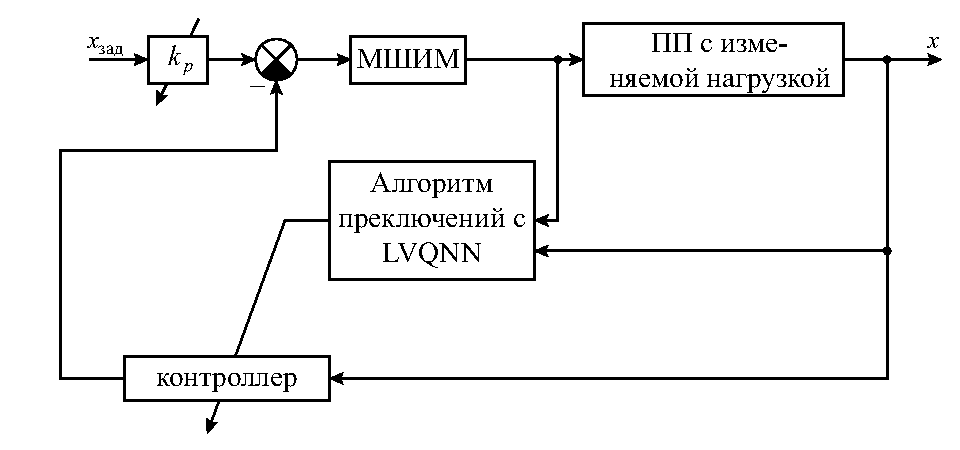
\includegraphics{mpwm_lvqnn.eps}
    \caption{Структурная схема системы управления с МШИМ и LVQNN}\label{fig:mpwm_lvqnn}
\end{figure}
с обратной связью по положению, скорости и ускорению. Такая структура обеспечивает высокое быстродействие и
точность позиционирования. Для адаптации параметров регулятора к изменяющимся внешним нагрузкам авторы применяют
нейронную сеть на основе векторного квантования (LVQNN). Данная интеллектуальная система классификации нагрузки
динамически подстраивает коэффициенты регулятора, компенсируя влияние возмущающих воздействий.

Проведённые экспериментальные исследования подтвердили, что предложенный алгоритм МШИМ обеспечивает точность позиционирования
в пределах \num{0.2}~\si{\milli\metre}, что существенно превосходит результаты стандартного ШИМ-алгоритма (ошибка около \num{1.75}~\si{\milli\metre}). Применение
LVQNN и адаптивной настройки параметров регулятора позволило эффективно компенсировать влияние изменяющейся внешней нагрузки и
добиться высокой стабильности системы управления.

Таким образом, ключевыми элементами разработанной системы управления являются алгоритм МШИМ,
трёхконтурная схема регулирования с обратной связью, а также интеллектуальная система адаптации параметров
регулятора на основе LVQNN. Полученные результаты демонстрируют высокую эффективность предложенных методов для точного
позиционного управления пневматическим пневмоприводом в условиях изменяющихся внешних нагрузок.


%%%%%%%%%%%%%%%%%%%%%%%%%%%%%%%%%%%%%%%%%%%%%%%%%%%%%%%%%%%%%%%%%%%%%%%%%%%%%%%%%%%%%%%%%%%%%%%%%%%%%%%%%%%%%%%%%%%%%%%%%%%%
%%%%%%%%%%%%%%%%%%%%%%%%%%%%%%%%%%%%%%%%%%%%%%%%%%%%%%%%%%%%%%%%%%%%%%%%%%%%%%%%%%%%%%%%%%%%%%%%%%%%%%%%%%%%%%%%%%%%%%%%%%%%
%%%%%%%%%%%%%%%%%%%%%%%%%%%%%%%%%%%%%%%%%%%%%%%%%%%%%%%%%%%%%%%%%%%%%%%%%%%%%%%%%%%%%%%%%%%%%%%%%%%%%%%%%%%%%%%%%%%%%%%%%%%%

\subsection{Исследование управления в скользящих режимах}\label{subsec:ch1/sec5/subsec2}

Управление в скользящих режимах \cite*{utkin2017sliding} -- это класс нелинейных методов управления, которые делают систему управления разрывной.
Процесс проектирования делится на два этапа: выбор поверхностей переключения для желаемого режима движения и синтез разрывного
управления для движения системы по этим поверхностям.

Движение системы по поверхностям переключения обладает рядом преимуществ: снижение порядка системы, инвариантность
к параметрическим и внешним возмущениям. Для описания движения используются специальные математические методы, такие
как регуляризация и метод эквивалентного управления.

Управление в скользящих режимах эффективно решает задачи управления сложными нелинейными динамическими объектами в
условиях неопределённости и широко применяется в электроприводах, робототехнике и системах автоматического управления.
Поскольку позиционный ПП с дискретными распределителями представляет из себя дискретную систему с релейным
управлением, то предостваляется воозможным использовать управление в скользящих режимах в ПП.

%%%%%%%%%%%%%%%%%%%%%%%%%%%%%%%%%%%%%%%%%%%%%%%%%%%%%%%%%%%%%%%%%%%%%%%%%%%%%%%%%%%%%%%%%%%%%%%%%%%%%%%%%%%%%%%%%%%%%%%%%%%%


В статье \cite*{Elsayed} рассматривается исследование, посвящённое управлению положением РО ПП
с использованием дискретных распределителей.

Авторы предлагают использование алгоритма управления скользящим режимом с коррекцией ошибки регулирования (SMCE), который использует
ШИМ для управления распределителями.

Для управления движением пневматического цилиндра авторы используют только три режима работы
четырёх распределителей, представленные ниже:
\begin{enumerate}
    \item Режим 1 -- выдвижение штока;
    \item Режим 2 -- задвижение штока;
    \item Режим 3 -- удержание положения штока;
\end{enumerate}

С целью оптимизации параметров SMCE и ПИД-регулятора была разработана модель в Simulink.
Экспериментальные исследования проводились на стенде ПП.

Результаты моделирования и экспериментов показывают, что SMCE обеспечивает более высокую точность
позиционирования, меньшее время установления и меньший выброс по сравнению с традиционным ПИД-регулятором.
Для гармонического входного сигнала среднеквадратичная ошибка при использовании SMCE составляет \num{0.22}~\si{\milli\metre}, а
для ПИД -- \num{0.69}~\si{\milli\metre}. Максимальная абсолютная ошибка для SMCE составляет \num{0.66}~\si{\milli\metre},
а для ПИД -- \num{1.46}~\si{\milli\metre}. Таким образом,
предложенный метод SMCE показал своё превосходство над ПИД-регулятором при управлении положением РО ПП.
%%%%%%%%%%%%%%%%%%%%%%%%%%%%%%%%%%%%%%%%%%%%%%%%%%%%%%%%%%%%%%%%%%%%%%%%%%%%%%%%%%%%%%%%%%%%%%%%%%%%%%%%%%%%%%%%%%%%%%%%%%%%

Статья \cite*{Hodgson:article1} аналогично посвящена разработке алгоритма управления в скользящих режимах
для регулирования ПП
с четырмя дискретными распределителями.

Ключевым отличием от предыдущих работ является расширение числа доступных дискретных режимов управления
с трех до семи.

В основе контроллера лежит скользящая поверхность $s$, которая определяется как функция ошибки позиционирования $e$,
её производной и второй производной. Авторы вводят семь возможных режимов переключения распределителей $(M_1 \div M_7)$,
выбор которых производится в зависимости от текущего значения $s$ и eё производной. Диаграмма переходов
представлена на рисунке.

\begin{figure}[ht]
    \centerfloat{
        \begin{tikzpicture}[auto]
            \usetikzlibrary {matrix,positioning,shapes.misc,arrows,shapes.geometric,graphs,backgrounds,arrows.meta}
            \tikzstyle{main_block} = [rectangle, rounded corners=0.5cm, draw, text centered, minimum height=4em, line width=1pt, text width=6em]
            \tikzstyle{text_block} = [rectangle, rounded corners=0.25cm, text centered, fill=white]
            \tikzstyle{cond_block} = [diamond, text centered, draw, text centered, line width = 1pt]
            \tikzstyle{arr} = [-triangle 45, line width=1pt]
            \tikzstyle{line} = [-, line width=1pt]
            % \tikzstyle{dashed} = [-triangle 45, line width=1pt, dashed]
            \matrix [column sep=3mm, row sep=7mm]
            {
                                                                              &
                                                                              &
                \node[main_block] (M7) {$M_7$\\$P_1$ -- оп.\\$P_2$ -- нап.};    \\
                %
                \node[text_block] (t1_0) {$\beta$};                           &
                \node[text_block] (t1_1) {$s > \beta$};                       &
                \node[text_block] (t1_2) {$s > \beta$};                       &
                \node[text_block] (t1_3) {$s > \beta$};                         \\
                %
                                                                              &
                \node[main_block] (M5) {$M_5$\\$P_1$ -- зап.\\$P_2$ -- нап.}; &
                \node[cond_block] (C1) {$E_1 > 1$};                           &
                \node[main_block] (M3) {$M_3$\\$P_1$ -- оп.\\$P_2$ -- зап.};    \\
                %
                \node[text_block] (t2_0) {$\epsilon$};                        &
                \node[text_block] (t2_1) {$s < \epsilon$};                    &
                \node[text_block] (t2_2) {$s > \epsilon$};                    &
                \node[text_block] (t2_3) {$s < \epsilon$};                      \\
                %
                                                                              &
                                                                              &
                \node[main_block] (M1) {$M_1$\\$P_1$ -- зап.\\$P_2$ -- зап.};   \\
                %
                \node[text_block] (t3_0) {$-\epsilon$};                       &
                \node[text_block] (t3_1) {$s > -\epsilon$};                   &
                \node[text_block] (t3_2) {$s < -\epsilon$};                   &
                \node[text_block] (t3_3) {$s > -\epsilon$};                     \\
                %
                                                                              &
                \node[main_block] (M2) {$M_2$\\$P_1$ -- нап.\\$P_2$ -- зап.}; &
                \node[cond_block] (C2) {$E_1 > 1$};                           &
                \node[main_block] (M4) {$M_4$\\$P_1$ -- зап.\\$P_2$ -- оп.};    \\
                %
                \node[text_block] (t4_0) {$-\beta$};                          &
                \node[text_block] (t4_1) {$s < -\beta$};                      &
                \node[text_block] (t4_2) {$s > -\beta$};                      &
                \node[text_block] (t4_3) {$s < -\beta$};                        \\
                %
                                                                              &
                                                                              &
                \node[main_block] (M6) {$M_6$\\$P_1$ -- нап.\\$P_2$ -- оп.};    \\
                %%%%%%%%%%%%%%%%%%%%%%%%%%%%%%%%%%%%%%%%%%%%%%%%%%%%%%%%%%%%%%%%%%%%
            };
            \begin{scope}[on background layer]
                \draw[arr] (M7.south) -- (C1);
                \draw[line] (M5.north) -- (t1_1);
                \draw[arr] (t1_1.north) to [out=90,in=180]  (M7.west);
                \draw[line] (M3.north) -- (t1_3);
                \draw[arr] (t1_3.north) to [out=90,in=0] (M7.east);

                \draw[arr] ([xshift=1cm]M5.north) to [out=90,in=90] node[below] {$\tau$} (C1.north);
                \draw[arr] ([xshift=-1cm]M3.north) to [out=90,in=90] node[below] {$\tau$} (C1.north);
                %%%%%%%%%%%%%%%%%%%%%%%%%%%%%%%%%%%%%%%%%%%%%%%%%%%%%%%%%%%%%
                \draw[line, loosely dashed] (t1_0.east) -- ([xshift=3cm]t1_3.west);
                \draw[line, loosely dashed] (t2_0.east) -- ([xshift=3cm]t2_3.west);
                \draw[line, loosely dashed] (t3_0.east) -- ([xshift=3.4cm]t3_3.west);
                \draw[line, loosely dashed] (t4_0.east) -- ([xshift=3.4cm]t4_3.west);

                \draw[line] (M5.south) -- (t2_1.north);
                \draw[line] (M3.south) -- (t2_3.north);
                %%%%%%%%%%%%%%%%%%%%%%%%%%%%%%%%%%%%%%%%%%%%%%%%%%%%%%%%%%%%%
                \draw[arr] (C1.west) -- (M5.east);
                \draw[arr] (C1.east) -- (M3.west);

                \draw[arr] (t2_1.south) to [out=-90,in=180]  (M1.west);
                \draw[arr] (t2_3.south) to [out=-90,in=0] (M1.east);

                \draw[arr] (M1.north) -- (C1.south);
                %%%%%%%%%%%%%%%%%%%%%%%%%%%%%%%%%%%%%%%%%%%%%%%%%%%%%%%%%%%%%

                \draw[arr] (M1.south) -- (C2);
                \draw[line] (M2.north) -- (t3_1);
                \draw[arr] (t3_1.north) to [out=90,in=180]  (M1.west);
                \draw[line] (M4.north) -- (t3_3);
                \draw[arr] (t3_3.north) to [out=90,in=0] (M1.east);

                \draw[arr] ([xshift=1cm]M2.south) to [out=-90,in=-90] node[above] {$\tau$} (C2.south);
                \draw[arr] ([xshift=-1cm]M4.south) to [out=-90,in=-90] node[above] {$\tau$} (C2.south);

                \draw[arr] (M6.north) -- (C2.south);

                \draw[line] (t4_1.north) --  (M2.south);
                \draw[line] (t4_3.north) --  (M4.south);

                \draw[arr] (t4_1.south) to [out=-90,in=180]  (M6.west);
                \draw[arr] (t4_3.south) to [out=-90,in=0] (M6.east);

                \draw[arr] (C2.west) -- (M2.east);
                \draw[arr] (C2.east) -- (M4.west);

                \draw[arr] ([xshift=-6cm]M6.south) -- node {$s$} ([xshift=-6cm]M7.north);

                % %%%%%%%%%%%%%%%%%%%%%%%%%%%%%%%%%%%%%%%%%%%%%%%%%%%%%%%%%%%%%
                % \draw[line, loosely dashed] (t1_0.east) -- ([xshift=3cm]t1_3.west);
                % \draw[line, loosely dashed] (t2_0.east) -- ([xshift=3cm]t2_3.west);
                % \draw[line, loosely dashed] (t3_0.east) -- ([xshift=3.4cm]t3_3.west);
                % \draw[line, loosely dashed] (t4_0.east) -- ([xshift=3.4cm]t4_3.west);
            \end{scope}
        \end{tikzpicture}
    }
    \caption{Диаграмма переключения режимов }\label{fig:actuators_scheme}
\end{figure}

Режимы $M_7$ и $M_6$ применяются при больших по модулю значениях $s$ для обеспечения максимальных ускорений в положительном и
отрицательном направлениях соответственно. Эти режимы позволяют быстро сократить большие ошибки позиционирования.

Режимы $M_2, M_3, M_4$ и $M_5$ используются при малых ошибках позиционирования $(\lvert s \rvert < \beta)$. Их применение позволяет снизить частоту
переключений распределителей, что способствует увеличению срока службы пневматической системы.

Для выбора оптимального режима в области малых ошибок авторы вводят дополнительные критерии, основанные на разности давлений
в камерах пневмопривода. Это позволяет определить режим, обеспечивающий максимальное ускорение при минимальном переключении
распределителей. Кроме того, вводится параметр $\tau$, задающий минимальное время между переключениями в этой области, что также
способствует снижению частоты переключений распределителей.

Теоретический анализ показывает, что при достаточно больших значениях параметров распределителей, предложенный алгоритм
обеспечивает асимптотическую устойчивость замкнутой системы. Результаты моделирования и экспериментальных исследований подтверждают,
что семирежимный скользящий контроллер демонстрирует улучшение точности позиционирования и значительное снижение переключений соленоидных
распределителей по сравнению с трехрежимным аналогом.

Таким образом, данная работа предлагает эффективное решение для управления пневматическими приводами с дискретными входами, обеспечивая
высокую точность позиционирования при сокращении нагрузки на исполнительные механизмы.

%%%%%%%%%%%%%%%%%%%%%%%%%%%%%%%%%%%%%%%%%%%%%%%%%%%%%%%%%%%%%%%%%%%%%%%%%%%%%%%%%%%%%%%%%%%%%%%%%%%%%%%%%%%%%%%%%%%%%%%%%%%%

Аналогично, в статье \cite*{Zhonglin} рассматривается разработка и проверка алгоритма управления в скользящем режиме с
использованием ШИМ для систем позиционирования в ПП. Этот алгоритм был так же применён к ПП с четырьмя дискретными распределителями.

Основная цель исследования заключалась в снижении ошибок позиционирования и повышении точности слежения. В статье подробно рассматриваются существующие подходы к управлению в ПП системах.

Разработанный алгоритм основан на использовании семи режимов переключения распределителей. В отличие от традиционных методов,
использующих высокое или низкое напряжение в одном периоде ШИМ, предложенная методика применяет два режима переключения за один период,
что улучшает производительность, комбинируя управление фазами ШИМ.

Статья подробно описывает процесс разработки алгоритма управления с использованием скользящего режима.
Он начинается с математической модели и заканчивается настройкой параметров и верификацией системы на платформе FPGA.
Использование FPGA в электропневматических системах является инновационным подходом. Авторы продемонстрировали эффективность
предложенного алгоритма как в математической модели, так и в экспериментальных условиях.

Экспериментальная часть включает настройку аппаратной части системы и платформы FPGA, а также тестирование на реальной установке.
Результаты подтвердили высокую точность и надёжность предложенного метода по сравнению с традиционными подходами.

Авторы подытоживают, что предложенный алгоритм обеспечивает высокую точность и устройчивость управления.
Предложенный алгоритм позволил уменьшить статическую ошибку позиционирования с \num{2.5}~\si{\milli\metre} до \num{0.8}~\si{\milli\metre},
что составляет снижение ошибки на \num{68}\%.
В свою очередь, точность позиционирования при математическом моделировании достигла \num{98.5}\% по сравнению с \num{91.2}\% при
использовании традиционных методов.

Кроме того, время отклика системы сократилось на 33\%, обеспечивая более высокое быстродействие. В
эксперименте отклонение при повторяющихся циклах позиционирования не превышало \num{1.2}~\si{\milli\metre}, тогда как
у традиционного алгоритма с ШИМ, это значение было в среднем \num{3.7}~\si{\milli\metre}.

\subsection{Исследование управления c применением интеллектуальных алгоритмов}\label{subsec:ch1/sec5/subsec3}

Интеллектуальные алгоритмы представляют из себя класс методов, основанных на применнении ИИ и МО для решения задач управления, в
которых требуется адаптация, обучаемость и предсказательность поведения в процессе функционирования. В отличии от классических методов,
интелектуальные методы способны анализировать поступающие данные, обучаться на их основе и принимать решения, основываясь на полученном или
накопленном опыте.

Можно выделить основные аспекты, которыми владееют интеллектуальные алгоритмы:
\begin{enumerate}
    \item способность к адаптации к изменяющимся условиям;
    \item способность к обучению на основе данных;
    \item способность к принятию решений на основе полученной информации;
    \item способность поиска оптимальных решений в условиях неопределённости.
\end{enumerate}

Одним из таких интеллектуальных алгоритмов является - нечеткая логика. Данный алгоритм
